% -----------------------------------------------
% Template for ISMIR Papers
% 2017 version, based on previous ISMIR templates

% Requirements :
% * 6+n page length maximum
% * 4MB maximum file size
% * Copyright note must appear in the bottom left corner of first page
% * Clearer statement about citing own work in anonymized submission
% (see conference website for additional details)
% -----------------------------------------------

\documentclass{article}
\usepackage{amsmath,cite,url}
\usepackage{graphicx}
\usepackage{color}

\newcommand{\ipt}{IPT}

\newcommand{\ml}[1]{\textcolor{blue}{ML : #1}}

% Title.
% ------
\title{Spontaneous Similarity Judgments of Musical Tones played with various Playing Techniques}

% Note: Please do NOT use \thanks or a \footnote in any of the author markup

% Single address
% To use with only one author or several with the same address
% ---------------
%\oneauthor
% {Names should be omitted for double-blind reviewing}
% {Affiliations should be omitted for double-blind reviewing}

% Two addresses
% --------------
%\twoauthors
%  {First author} {School \\ Department}
%  {Second author} {Company \\ Address}

%% To make customize author list in Creative Common license, uncomment and customize the next line
%  \def\authorname{First Author, Second Author}


% Three addresses
% --------------
\author{Mathieu Lagrange, Christian EL-Hajj, Mathias Rossignol, Grégoire Lafay}

%% To make customize author list in Creative Common license, uncomment and customize the next line
%  \def\authorname{First Author, Second Author, Third Author}

% Four or more addresses
% OR alternative format for large number of co-authors
% ------------
%\multauthor
%{First author$^1$ \hspace{1cm} Second author$^1$ \hspace{1cm} Third author$^2$} { \bfseries{Fourth author$^3$ \hspace{1cm} Fifth author$^2$ \hspace{1cm} Sixth author$^1$}\\
%  $^1$ Department of Computer Science, University , Country\\
%$^2$ International Laboratories, City, Country\\
%$^3$  Company, Address\\
%{\tt\small CorrespondenceAuthor@ismir.edu, PossibleOtherAuthor@ismir.edu}
%}
%\def\authorname{First author, Second author, Third author, Fourth author, Fifth author, Sixth author}


\sloppy % please retain sloppy command for improved formatting

\begin{document}
%
\maketitle
%
\begin{abstract}

Musical timbre is a multi-faceted notion that have been extensively studied, mostly focusing on its spectral aspect. By studying the spontaneous judgments of similarity between several instruments played with a diverse set of playing techniques, we aim in this paper at better understanding the influence of the change of the playing technique on the perception of timbre.

A first experiment is conducted by music experts to identify which couple of instrument and playing technique in a given dataset is worth comparing to other couples of instrument / playing technique. In a second experiment, spontaneous similarity judgments among the retained couples are collected using a canonic free sorting task experiment design.


To further study the outcomes of this experiment, we assume a two-step computational model of human perception, where the acoustic signal is fed to a statically designed processing unit that accounts for frequency and temporal modulations. The resulting features are then projected using a supervised technique which considers as input the perceptual similarity judgments gathered in the second experiment. Numerical experiments show that the induced perceptual space is able to approximate perceptual data with satisfying accuracy.

\end{abstract}
%
\section{Introduction}\label{sec:introduction}

Musical timbre is an interesting notion to study as it is perceptively defined. Thus, by studying musical timbre, one study many facets of the human auditory system which responds to a diverse -- but somewhat more controled than other stimuli such as speech or environemntal sounds -- set of physical stimuli.

A popular view of the kind of stimuli we consider is that they can be described by a spread of energy that evolve through time and across frequency. By following this trend, most researchers translate the negation of the ASA definition of timbre into a more relative definition : musical timbre is about the distribution of intensity across the time / frequency plane.

A great deal of litterature focuses on the instaneous spectrum, \textit{i.e.} the timbre can be defined without considering evolution of the energy distribution trough time. Other studies demonstrated the importance of the onset in the recognition of some musical instruments. Those studies on a rather short term model where the waveform is observed in a range that do not exceed 100 ms.

Interestingly, modern physiological models of the primary mamalian auditory system also considers the evolution of the energy distribution at longer time scales, \textit{i.e.} how the energy modulates through time for given frequencies.  Dau's model acount for frequency and rate of modulation. Shamma's model account for frequency, rate and bandwidth to fully describes the physiological evidence gathered by studying the auditory system of the ferret. Though, most of the numerical experiments done using this model did not fully demonstrated the usefullness of this third dimension.

Thus, by taking a signal processing view of the matter, one could consider that a first stage of the auditory system proceeds to a rather fixed set of convolutions across time and frequency, projecting the signal into a large set of descriptive features organized across frequency and rate of modulations.

What the higher level of the auditory cortex does remains largely unkown, but we can assume that the level of plasticity is very high, as any living entity has to adapt their percepts to a wide diversity of tasks.  Considering the lack of information about this stage, we will assume in this paper that this second step is rather opportunistic, in the sense that, from this large set of features, it aims at multiplexing in some way the ones that are the most relevant for the task at hand.

Considering not only the type of musical instrument but also the playing technique is interesting in that matter, as it invite us to consider the relation between the rate of modulation and timbre percepts. A notion that have not been extensively studied in the litterature. It also permits to consider the notion of timbral similarity at finer grain of detail.

The contributions of the paper are as follows: 1) provide perceptual data that account for the perception of musical tones played with various playing techniques, 2), demonstrate that, for the gathered data, the type of playing technique plays an important role for the organization of the data, and 3) propose a perceptually motivated computational model of timbre perception that account well for the human judgments studied in this paper.



\section{Experiment 1}\label{sec:}


The dataset considered in this study has audio recording of 16 different  musical instruments () played with different playing techniques, which leads to 143 different couple of instrument / playing technique. For each couple, the pitch and intonation is varied leading to 25444 samples. The way the dataset is segmented is explained in more details in Appendix \ref{sec:dataset}.

Studies about perceptual similarity are plagued with a dimensional problem. When considering $n$ items, a complete exploration of the similarity space requires the filling of a $n^2$ matrix. Assuming a symmetric similarity (the similarity of A to B is equl to the similarity of B to A) reduces the number but not by much.

In an attempt to reduce the number of items, we decided to perform a selection experiment where the subject is asked to give his opinion on which \ipt is relevant to study. An \ipt is said to be relevant to study if it is likely to be associated to another \ipt. Interest is rated on a 7 ticks scale. The subject can listen to all the different nuance and pitch samples of each \ipt. The experiment is over when all the \ipt have been rated.

Rating examples are given :
\begin{itemize}
  \item One star: this \ipt is singular, it is not useful to compare it with another \ipt.
  \item Four stars: there is a proximity on one aspect of the sound between this \ipt and of an \ipt of another instrument, but this one is neither decisive nor obvious.
  \item Seven stars: there is a large similarity between this \ipt and an \ipt of another instrument, it is interesting to keep it.
\end{itemize}

Two musical composition professors of the CNSMDP, a renowned French school of music performed the test. All the couples with a grade higher than three are selected, bringing 78 \ipt to study.

\section{Experiment 2}\label{sec:}

The second experiment aims at gathering spontaneous judgment of similarity. We chose a canonical free sorting task  for several reasons. First, it gives the ability to the subject to listen to the whole set of \ipt before performing the task. Second, it gives more freedom to the subject thus potentially more interest to perform the task than a lengthy series of triplet dissimilarity ratings.

The subjects are thus asked to organize the 78 \ipt displayed as grey dots on a two dimensional plane into groups by assigning colors to each dots according to their acoustic similarity. The \ml{consigne} is deliberately vague in order to allow the subject to \ml{use its own representation of similarity}. The experiment is over when the sujbect assigned a color to all the dots. The initial location of the dots on the plane is randomized for each subject and can be changed during the experiment by the subject for convenience. Eventhough the location of the dots is recorded, this data is not considered during the analysis.

The experiment was available online for two months and requests to perform the test have been sent to internal mailing lists of the CNSMDP and international research mailing with a focus on audio and music processing. The experiment have been performed on a volountary basis without gratification.

\section{Analysis}\label{sec:}

\begin{figure}
\center
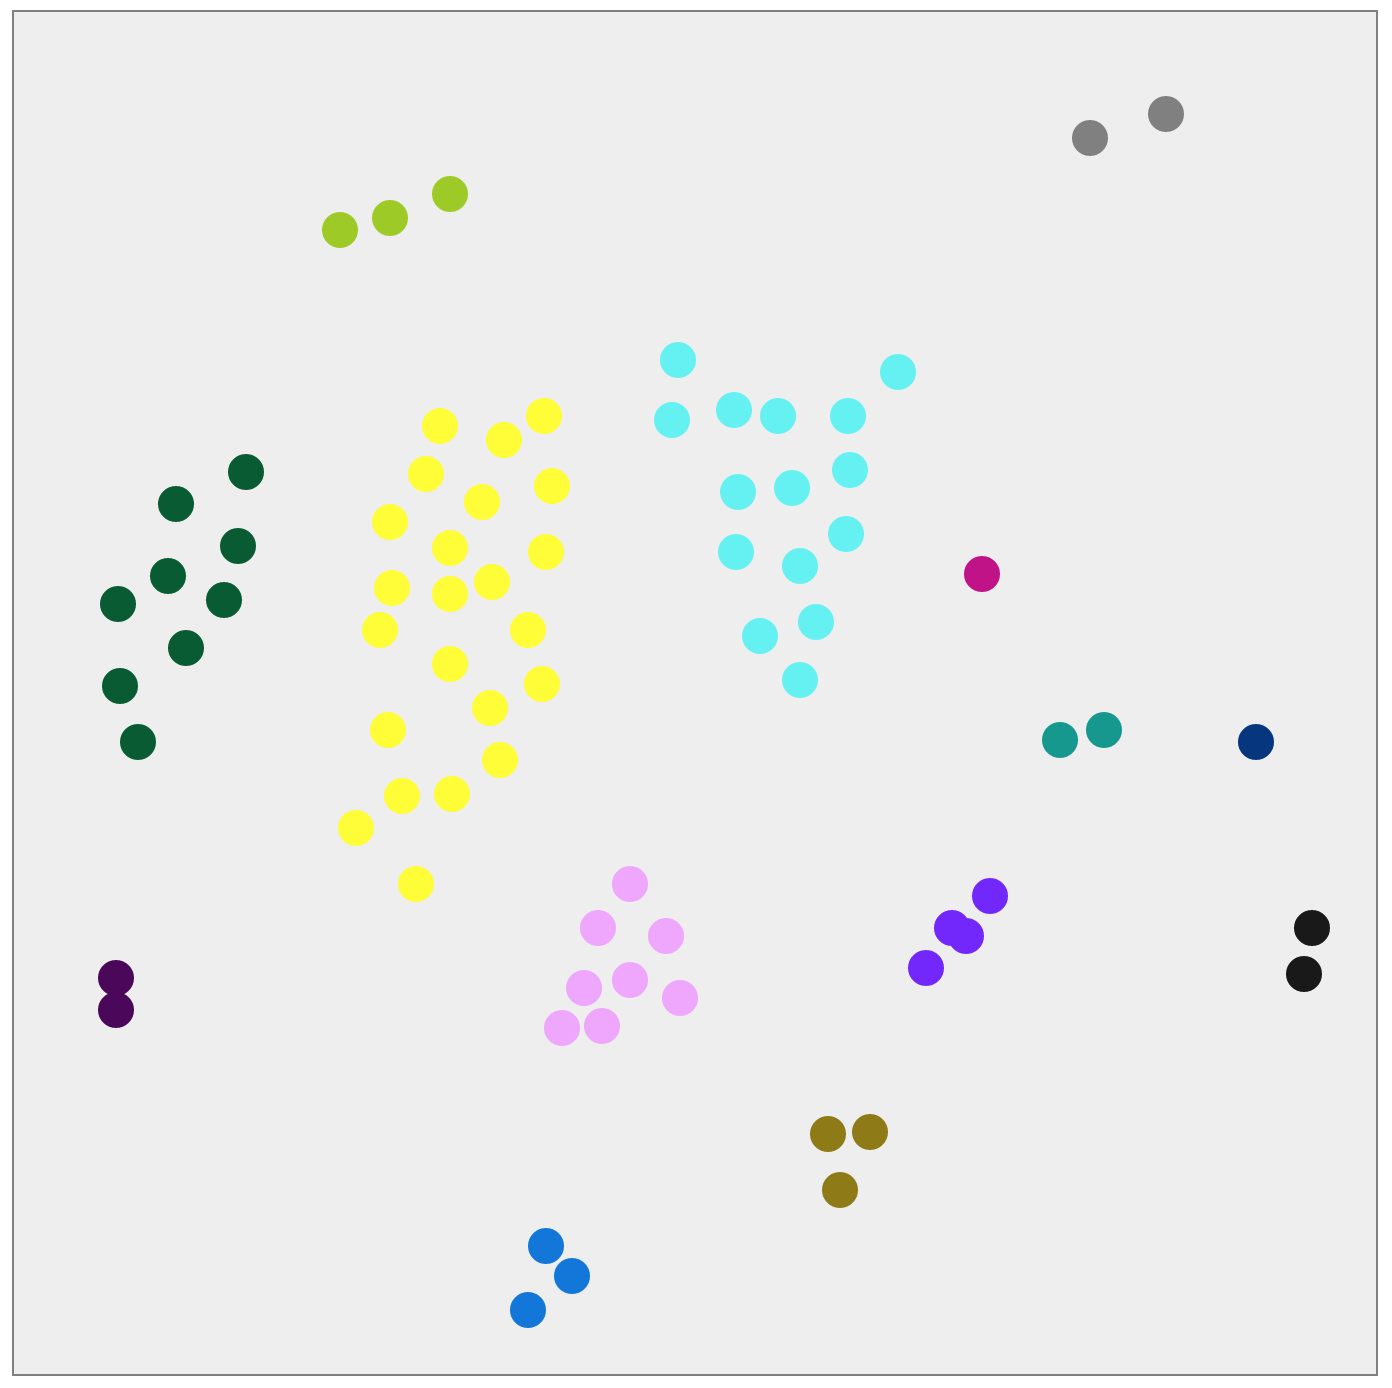
\includegraphics[width = \textwidth]{figures/xp2example.png}
\caption{Spatial and group organization provided by subject 1.}
\label{fig:xp2display}
\end{figure}

31 subjects completed the experiment. An example of resulting organisation of \ipt is given on Figure \ref{fig:xp2display}.  The resulting organisation for each subject are available for reader's inspection using the full feature interface provided to the subjects for performing the experiment\footnote{https://mathieulagrange.github.io/paperSpontaneousSimilarity/demo}.


As discussed in the previous section, only the grouping done using the colors is considered. The spatial organisation could provide information about the notion of similarity, but implicitely force the fact that the similarity space is two dimensional. We therefore now study the properties of the groupings performed by the subject prior converting them into an overall similarity matrix.

Among the 20 colors available, the subjects used on average \ml{fill}. The distribution of the number of groups can be seen on Figure \ref{fig:xp2nbGroup}. The size of the groups is on average \ml{fill}. The distribution of the size of groups can be seen on Figure \ref{fig:xp2sizeGroup}.

\begin{figure}
\center
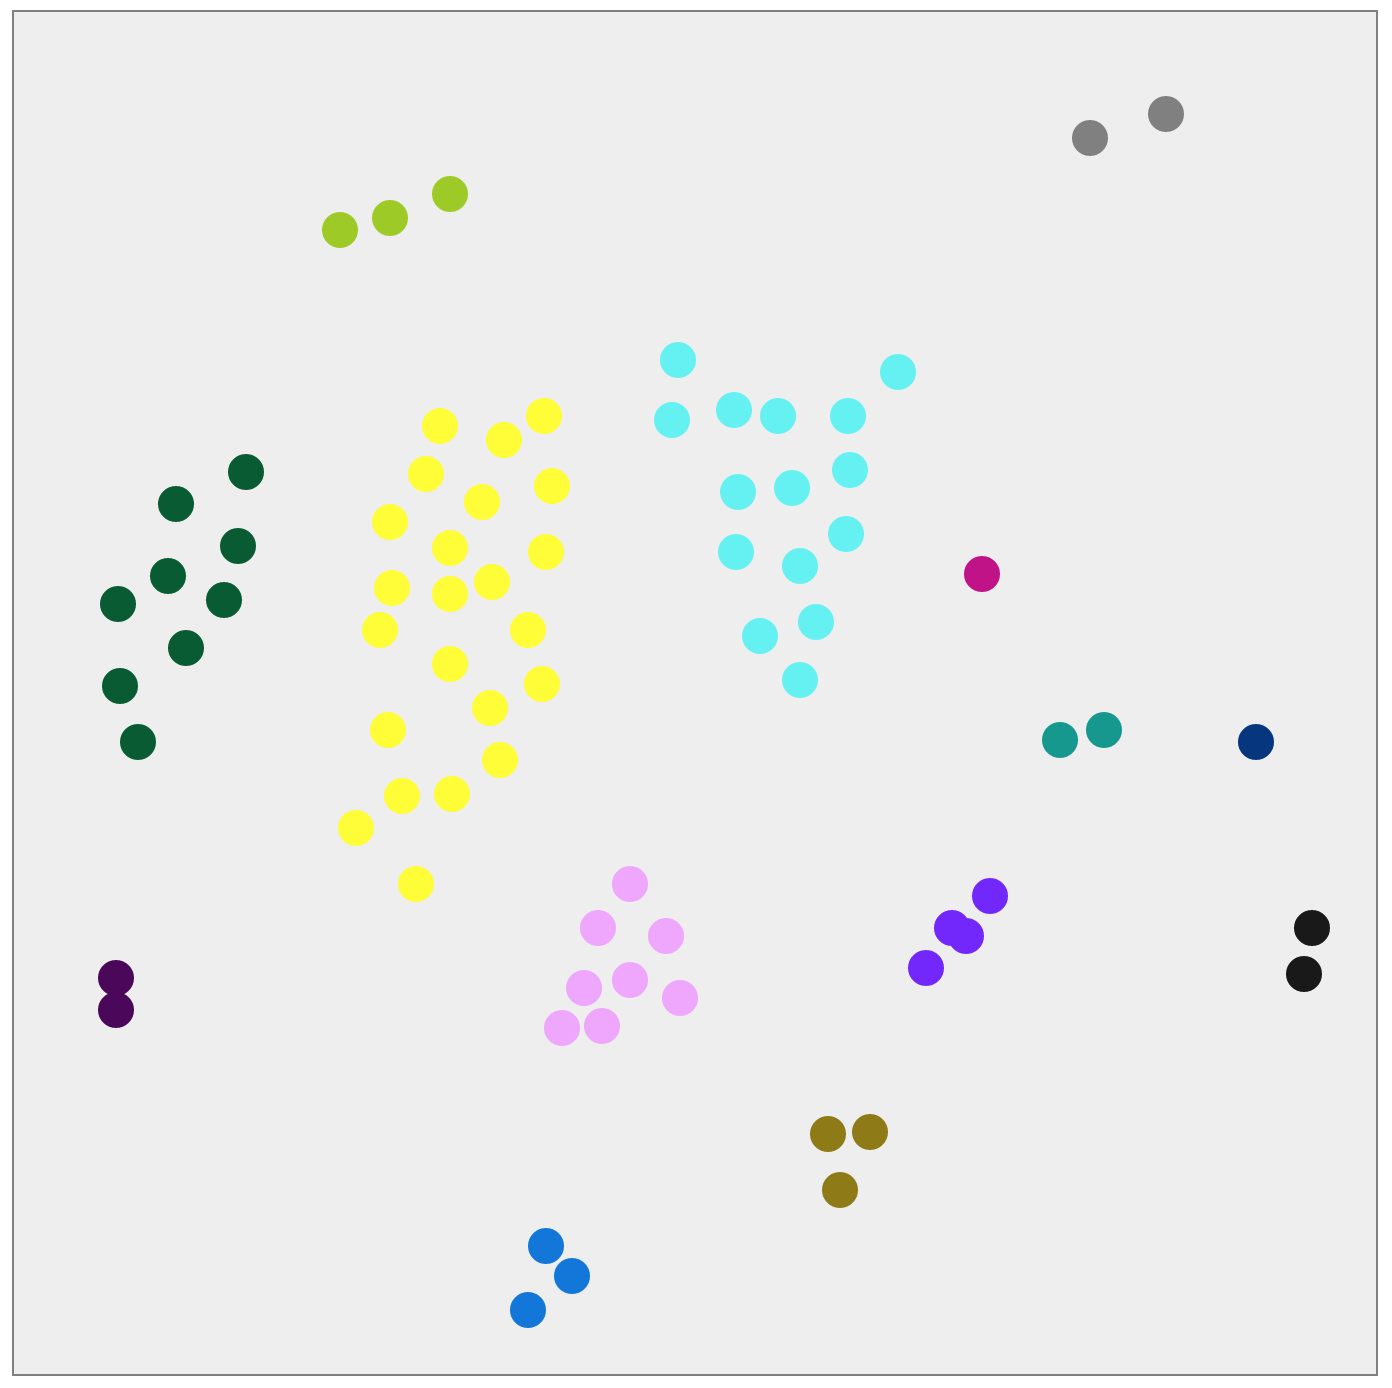
\includegraphics[width = \textwidth]{figures/xp2example.png}
\caption{Histogram of the number of groups.}
\label{fig:xp2nbGroup}
\end{figure}

\begin{figure}
\center
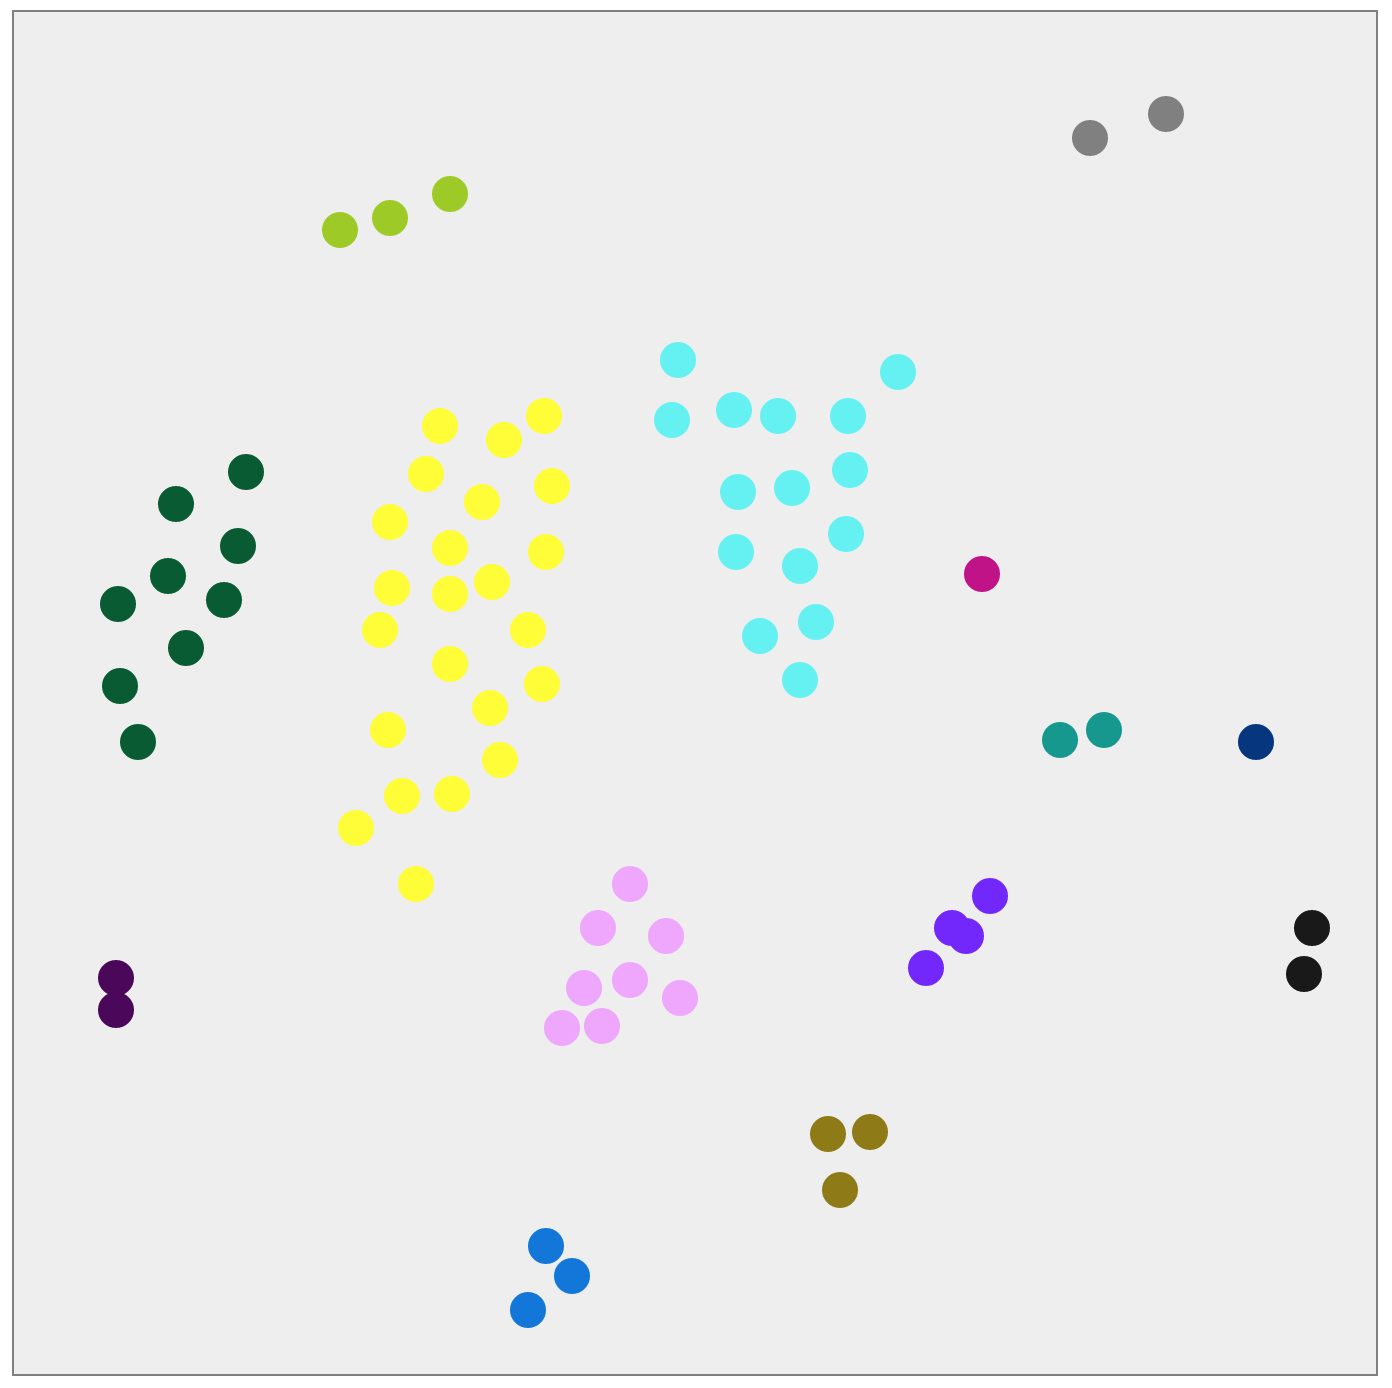
\includegraphics[width = \textwidth]{figures/xp2example.png}
\caption{Histogram of the size of groups.}
\label{fig:xp2sizeGroup}
\end{figure}

\begin{figure}
\center
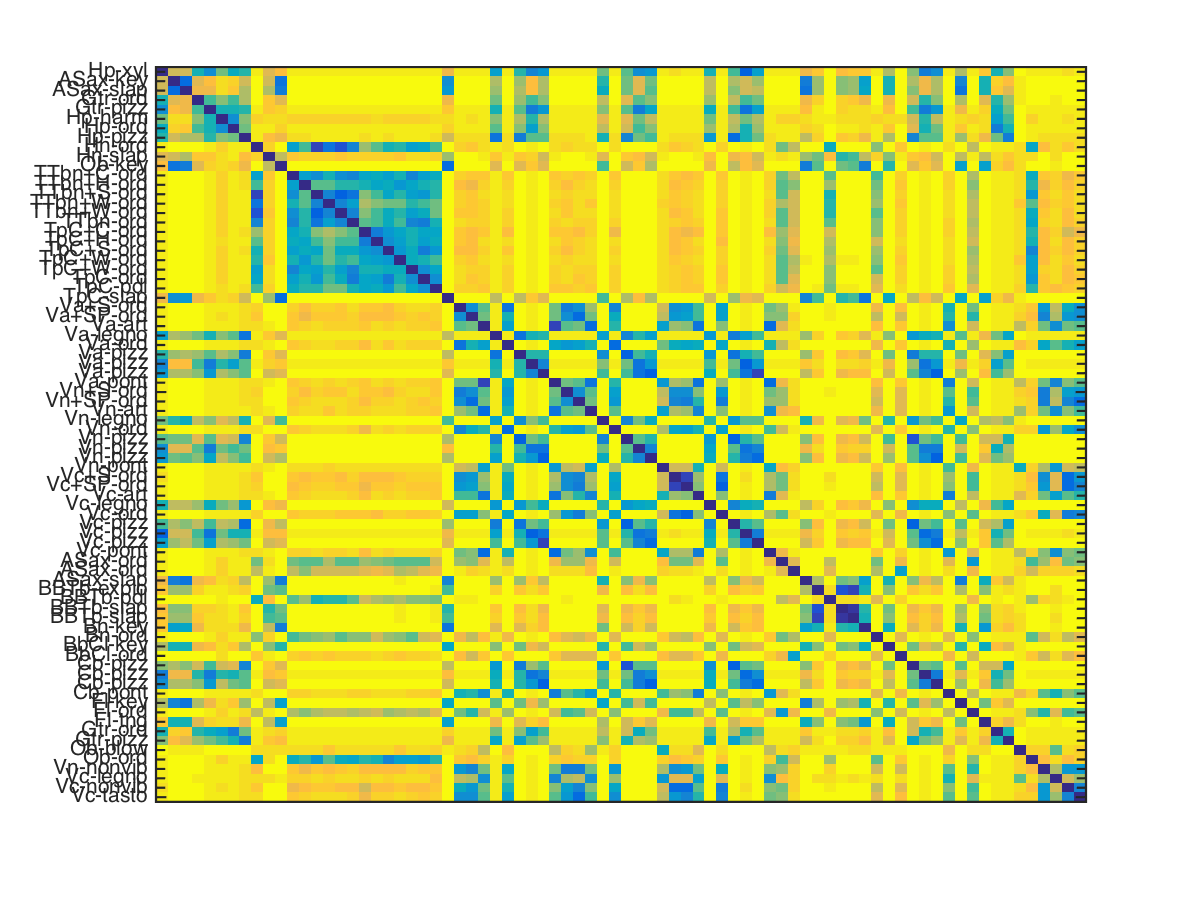
\includegraphics[width = \textwidth]{figures/allSim.png}
\caption{Binary similarity matrix corresponding to the grouping of subject 1.}
\label{fig:xp2sizeGroup}
\end{figure}

\begin{figure}
\center
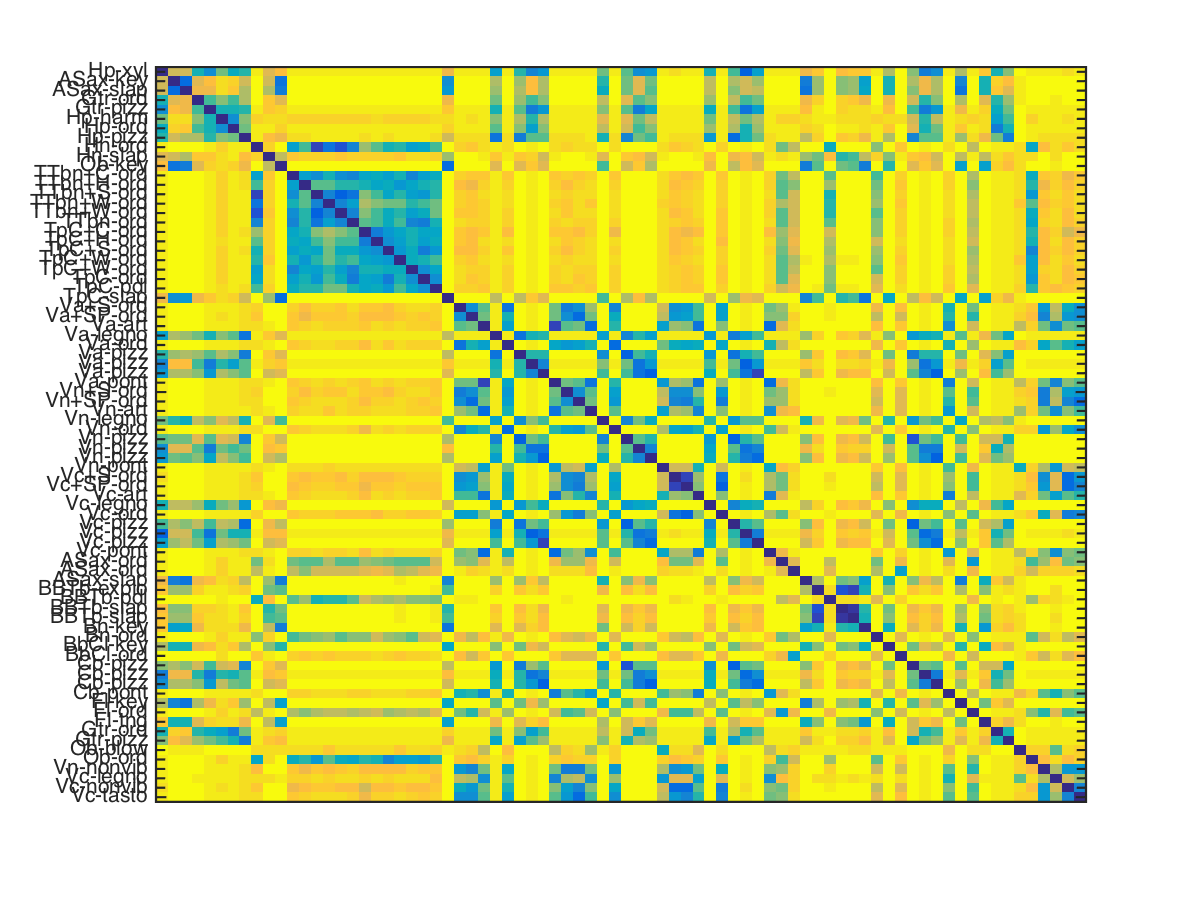
\includegraphics[width = \textwidth]{figures/allSim.png}
\caption{Average similarity matrix corresponding to the grouping of the complete cohort.}
\label{fig:xp2sizeGroup}
\end{figure}

\begin{figure}
\center
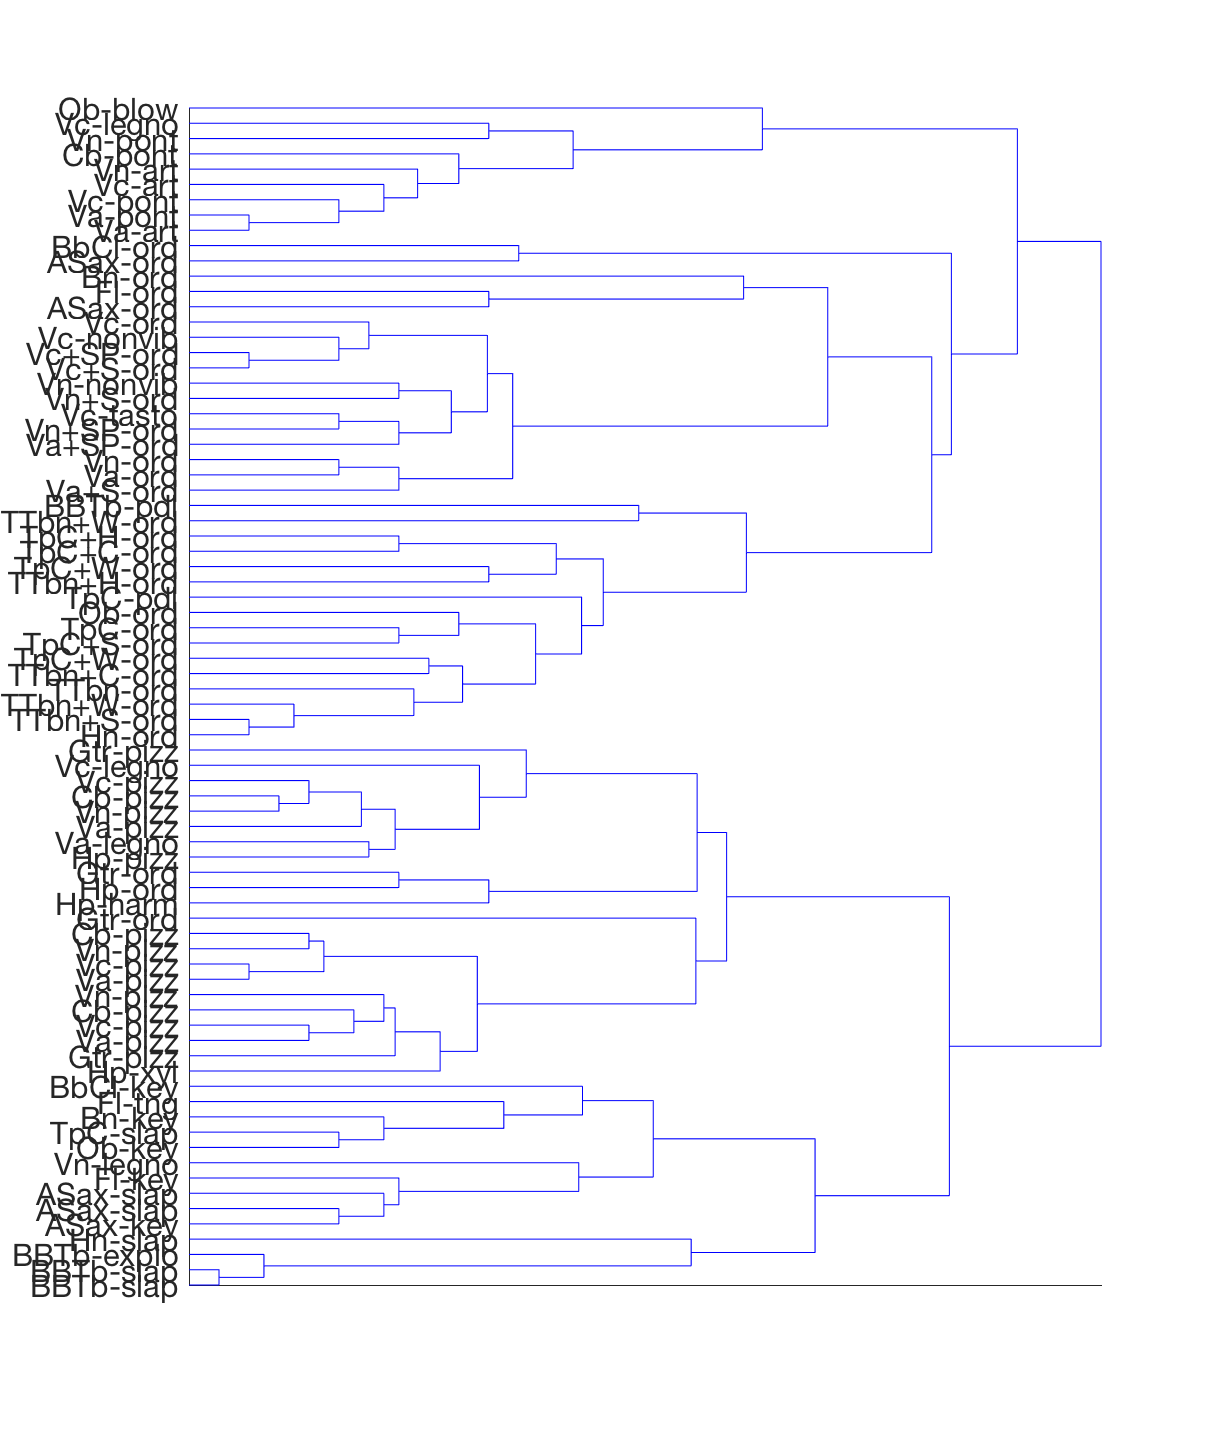
\includegraphics[width = \textwidth]{figures/allLinkage.png}
\caption{Dendrogram computed using the average similarity matrix.}
\label{fig:xp2sizeGroup}
\end{figure}

\begin{figure}
\center
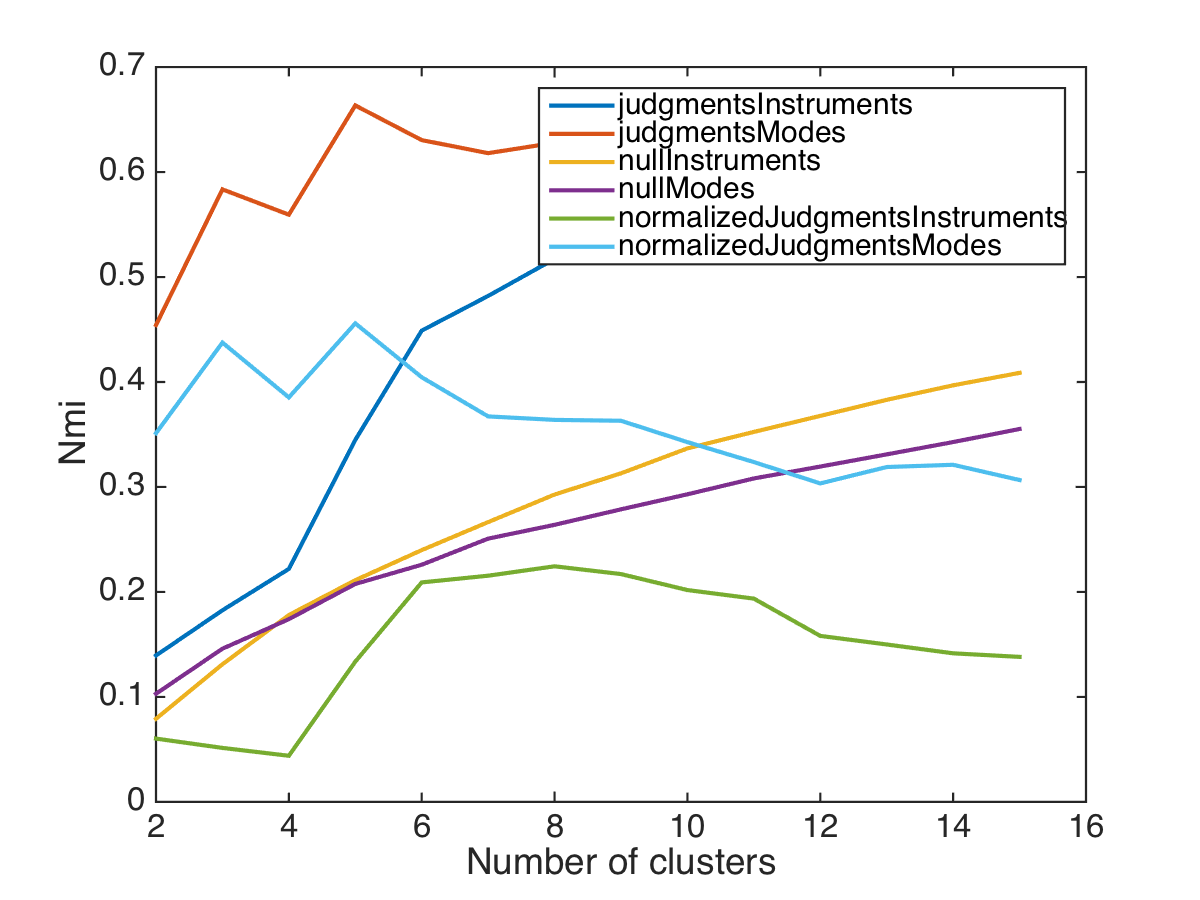
\includegraphics[width = \textwidth]{figures/clusterAnalysis.png}
\caption{Dendrogram computed using the average similarity matrix.}
\label{fig:xp2sizeGroup}
\end{figure}

\begin{figure}
\center
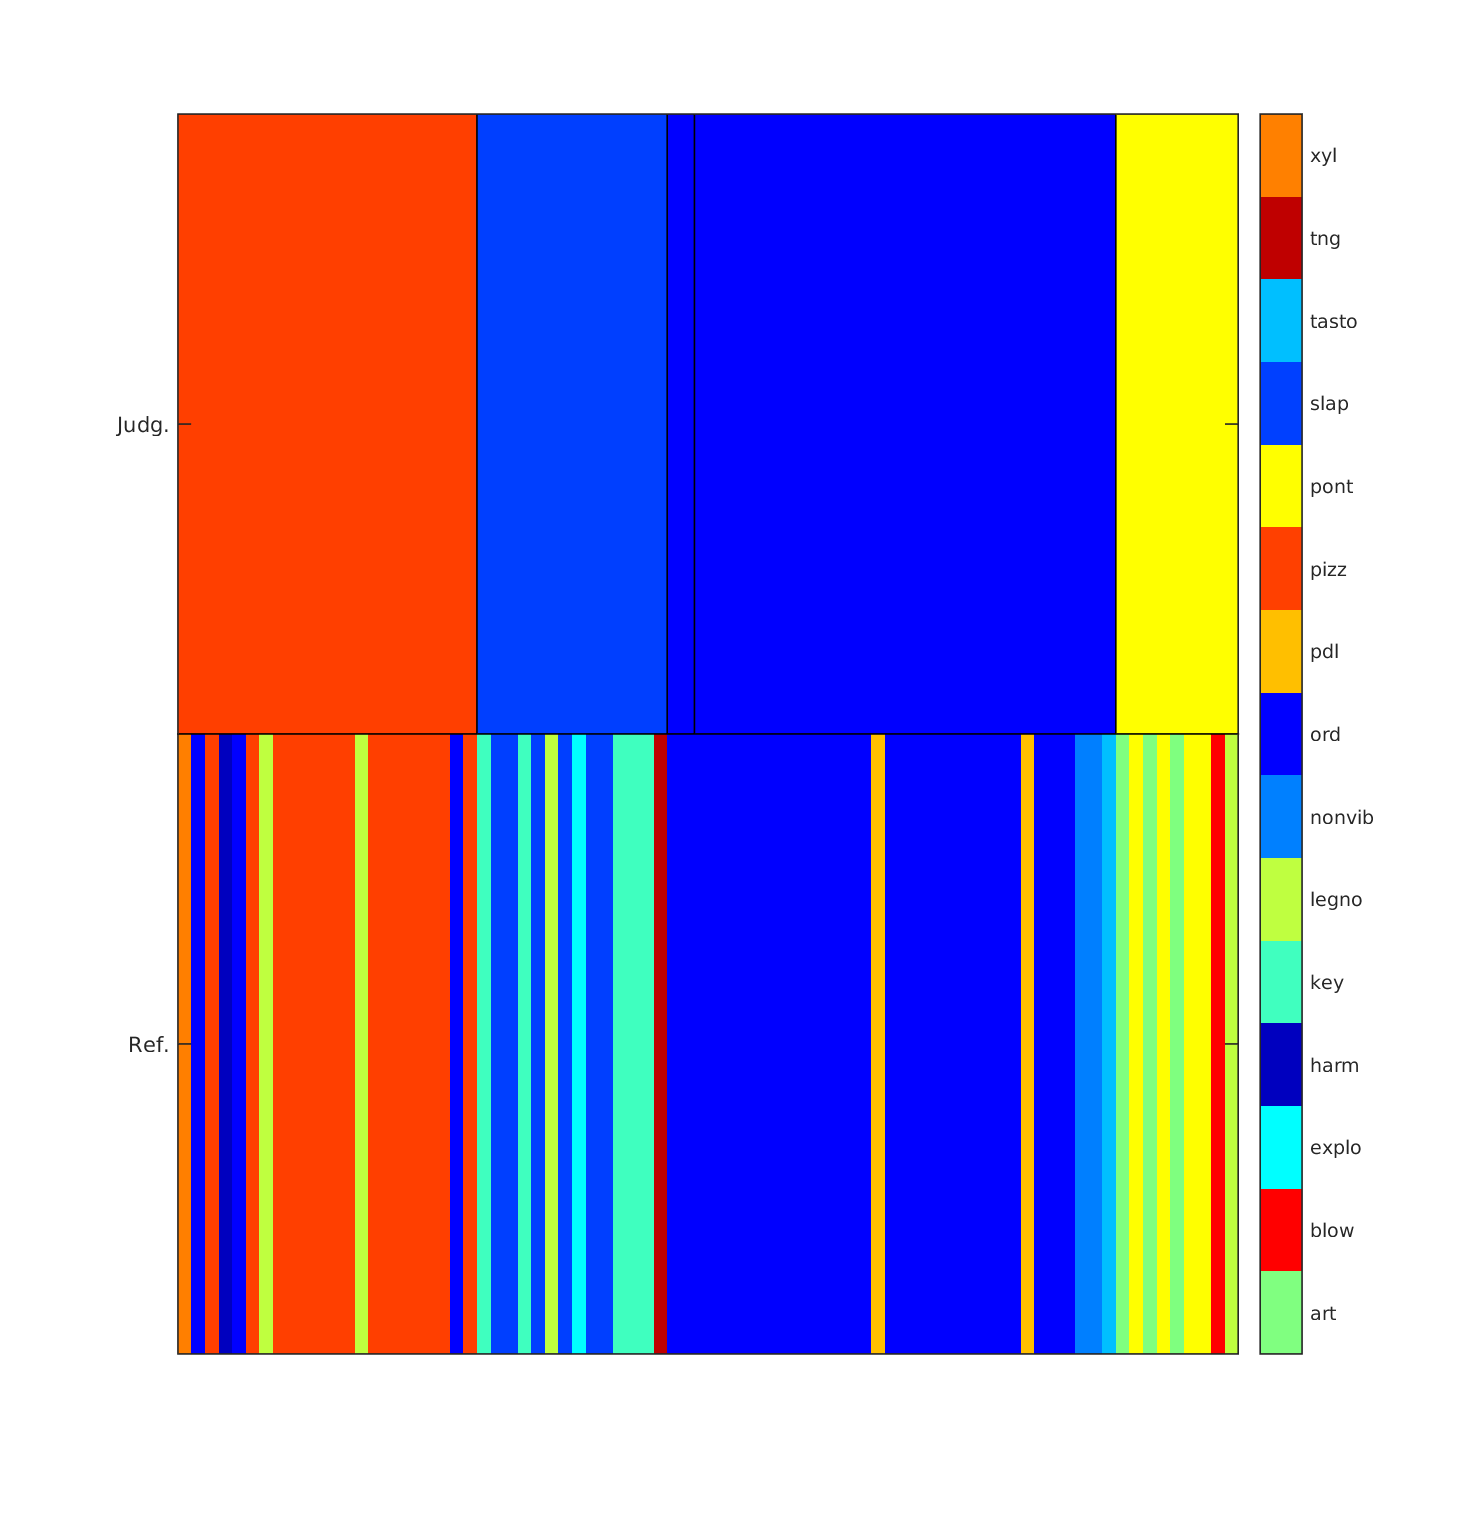
\includegraphics[width = \textwidth]{figures/groupModes.png}
\caption{Clustering \ipt using average perceptual similarity into 5 clusters (a) and playing technique labels (b). The colors of clusters displayed on top corresponds to the playing technique label that is dominant in this cluster.}
\label{fig:xp2sizeGroup}
\end{figure}

\begin{figure}
\center
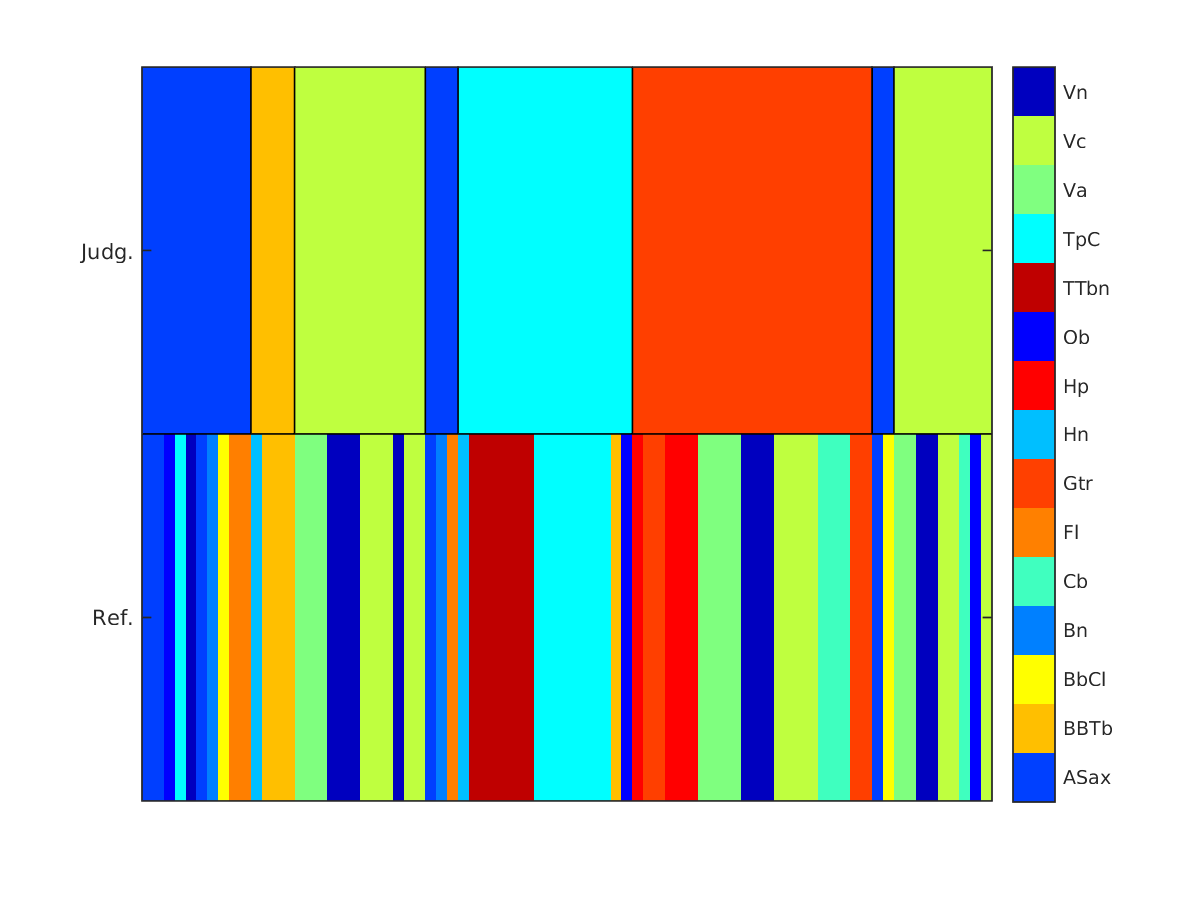
\includegraphics[width = \textwidth]{figures/groupInstruments.png}
\caption{Clustering \ipt using average perceptual similarity into 8 clusters (a) and instrument reference labels (b). The colors of clusters displayed on top corresponds to the playing technique label that is dominant in this cluster.}
\label{fig:xp2sizeGroup}
\end{figure}

\section{Model}\label{sec:}

\section{Results}\label{sec:}

\section{Discussion}\label{sec:}




% For bibtex users:
\bibliography{bib}

\section{Dataset}


% For non bibtex users:
%\begin{thebibliography}{citations}
%
%\bibitem {Author:00}
%E. Author.
%``The Title of the Conference Paper,''
%{\it Proceedings of the International Symposium
%on Music Information Retrieval}, pp.~000--111, 2000.
%
%\bibitem{Someone:10}
%A. Someone, B. Someone, and C. Someone.
%``The Title of the Journal Paper,''
%{\it Journal of New Music Research},
%Vol.~A, No.~B, pp.~111--222, 2010.
%
%\bibitem{Someone:04} X. Someone and Y. Someone. {\it Title of the Book},
%    Editorial Acme, Porto, 2012.
%
%\end{thebibliography}

\end{document}
